%%  export TEXINPUTS=.:/home/mjw/src/manuals/common:

\documentclass[11pt,a4paper,openany,oneside]{book}

\usepackage{hyperref} 
\usepackage{listings}
\usepackage{graphicx}

\newcommand{\ci}[1]{\hspace*{1cm} {\small\texttt{#1}}}
\newcommand{\cc}[1]{{\small\texttt{#1}}}

\newenvironment{description*}%
  {\setlength{\parskip}{0pt}%
	 \begin{description}%
		\setlength{\topsep}{-12pt}%
		\setlength{\itemindent}{-12pt}%
    \setlength{\itemsep}{0pt}%
		\setlength{\itemsep}{0pt}}%
  {\end{description}}

\newenvironment{enumerate*}%
  {\begin{enumerate}%
		\setlength{\topsep}{-12pt}%
		\setlength{\itemindent}{-12pt}%
    \setlength{\itemsep}{0pt}%
		\setlength{\parindent}{0pt}}%
  {\end{enumerate}}
  
\begin{document}

\begin{titlepage}

\begin{center}
{\Huge OpenTTP manual}
\end{center}

\vspace*{4cm}
\begin{center}
Version 1.0
\end{center}

\begin{center}
Copyright 2016 OpenTTP
\end{center}

\end{titlepage}

\tableofcontents
\listoffigures
\listoftables

\lstset{
	xleftmargin=24pt,
	basewidth=0.5em,
	basicstyle=\ttfamily,
	escapechar=\%
}

%% ****************************************************************************************
\chapter{Introduction}
%% ****************************************************************************************

\section{What is OpenTTP?}

\section{GPS common-view}

\section{The OpenTTP reference platform}

\section{Supported hardware}

	\subsection{GNSS receivers}
	
	\begin{description*}
		\item[Javad] (older, GRIL receivers)
		\item[Trimble] Resolution T
		\item[NVS] NV08
		\item[ublox] Neo8MT
	\end{description*}
	
	Note: OpenTTP uses a custom file format for logging GPS receiver data. It does not read native receiver binary-format files.
	
	Guidance on testing a receiver for suitability for time-transfer, and writing software to process
	the receiver's data, is given in the OpenTTP Developer's Guide.
	
	\subsection{Counter/timers}
	
	\begin{description*}
		\item Agilent 5313x, using IOTech GPIB to RS232 converter
		\item SRS PRS10 (using the input 1 pps time-tagging function)
		\item OpenTTP multichannel counter
	\end{description*}
	
%% ****************************************************************************************
\chapter{Getting started}
%% ****************************************************************************************

\section{Software installation requirements}

In addition to a basic Linux development environment, you will need the development packages for:
\begin{description*}
	\item[\cc{boost}]   
	\item[\cc{libgsl}] GNU scientific library
\end{description*}

Depending on your Linux installation, you may also need
\begin{description*}
	\item[\cc{Time::HiRes}] Perl library
\end{description*}

\section{Building and installing the software}

Two scripts are provided for installing the software.
\begin{lstlisting}
software/system/installsys.pl
software/gpscv/install.pl
\end{lstlisting}

\cc{installsys.pl} must be run first, because it installs libraries which are needed by the GPSCV software.

Run-time options can be viewed by running the script with the '-h' option. In particular, \cc{installsys.pl}
has options to list the available installation targets and to install particular targets.

\section{A minimal software setup}

Some users may only be interested in the core software that OpenTTP provides so that they can use
it with their own hardware. This section describes the minimum setup required for operation.

\subsection{Software}

The OpenTTP software is comprised of various C/C++ applications and Perl scripts.

You will need:
\begin{description*}
	\item \cc{TFLibrary.pm}
	\item \cc{libconfigurator}
	\item \cc{lockport} utility to create a UUCP lock file
	\item \cc{mktimetx} creates time-transfer files
	\item one of the OpenTTP-provided scripts to log your receiver
	\item one of the OpenTTP-provided scripts to log your counter/timer
\end{description*}

You must use one of the OpenTTP receiver logging scripts because \cc{mktimetx} expects a custom file-format. In particular, the
receiver's native binary formats are not readable by \cc{mktimetx}. Similarly, OpenTTP uses a custom file
format for the counter-timer measurement files, although in this case, conversion from another format
will probably be straight-forward. Most likely users will have to provide their own software for
logging their counter/timer, given the large number of possible devices here, and the limited
support within OpenTTP.

You may find the following useful:
\begin{description*}
	\item[kickstart.pl] for automatic start of logging processes
	\item[runmktimetx.pl] for automated processing, and reprocessing
	\item[ziplogs.pl] for log file compression
\end{description*}	

Sample configuration files can be found in \cc{software/gpscv/common/etc}.
The user running the logging and processing needs the following directories (or equivalents - most paths
can be configured via the general configuration file, \ref{sgpscvconf}.

\begin{description*}
	\item[\cc{bin}]
	\item[\cc{cggtts}]
	\item[\cc{etc}]
	\item[\cc{logs}]
	\item[\cc{raw}]
	\item[\cc{rinex}]
	\item[\cc{tmp}]
\end{description*}

%% ****************************************************************************************
\chapter{System hardware}
%% ****************************************************************************************

\section{Multi-channel counter/timer}

\begin{figure}
\centerline{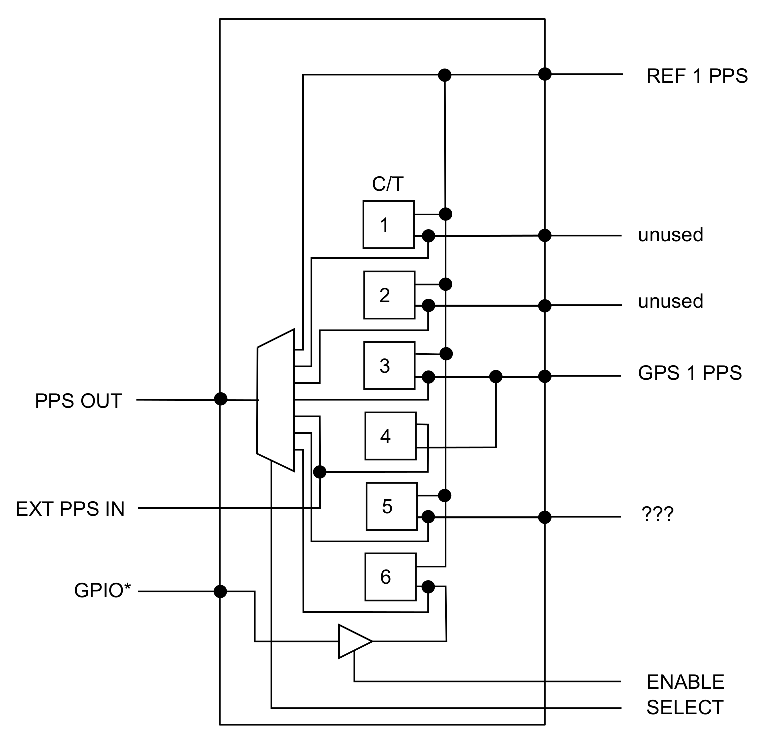
\includegraphics{figures/ottpcounter.eps}}
\end{figure}

\begin{table}
\begin{center}
\begin{tabular}{ll}
1 & channel 1 pps (unused)\\
2 & channel 2 pps (unused) \\
3 & channel 3 pps (GPS receiver)\\
4 & channel 4 pps (external pps)\\
5 & channel 5 pps (unused)\\
6 & channel 6 pps (GPIO)\\
7 & GPIO enabled\\
8 & Digital Clock Manager PLL is locked\\
\end{tabular}
\end{center}
\caption{Status LEDs}
\end{table}


%% ****************************************************************************************
\chapter{GPSCV software}
%% ****************************************************************************************

\section{Configuration file format \label{sConfigFileFormat}}

Configuration files use a common format and are plain text files, designed to be easily edited via a command-line
editor because in many applications, only shell access to the system will be available.

The file is divided into sections, with section names delimited by square brackets [ ]. Entries in each section
are of the form:
\begin{lstlisting}
	 key = value
\end{lstlisting}
For example,
\begin{lstlisting}
	 [Receiver]
	 manufacturer = Trimble
	 model = Resolution T
\end{lstlisting}
defines a section `Receiver' and the receiver's manufacturer and model. 
We use the notation \cc{Section::Key} to describe keys. For example,
\cc{Receiver::model} and \cc{Receiver::manufacturer} describe the two keys above.

Keys are not case-sensitive. Comments begin with a '\#'.

Some entries define a list of sections. For example, the comma-separated list of values for 'outputs' 
\begin{lstlisting}
	[CGGTTS]
	outputs = C1-code,P1-code,P2-code
\end{lstlisting}
defines three sections: \cc{C1-code}, \cc{P1-code}, and \cc{P2-code}.


\section{gpscv.conf - the core configuration file \label{sgpscvconf} }

A single configuration file, \cc{gpscv.conf}, provides configuration information to most of the
OpenTTP software. 
gpscv.conf is used by mktimex, receiver logging scripts, TIC logging scripts,receiver utilities and so on.

It uses the format described in \ref{sConfigFileFormat}.
\section{mktimetx}

\cc{mktimetx} is the core OpenTTP application. It creates CGGTTS and RINEX-format time-transfer files.


\section{runmktimetx.pl \label{runmktimetx}}


\section{runmktimetx.pl \label{runmktimetx}}

\hypertarget{h:runmktimetx}{}

\cc{runmktimetx.pl} provides a convenient way to process multiple days of data and to run any missed processing.

\cc{runmktimetx.pl} uses \cc{gpscv.conf}. There are no entries in \cc{gpscv.conf} specific to \cc{runmktimetx.pl}

\cc{runmktimetx.pl} doesn't produce a log file.
	
\subsection{usage}
\cc{runmktimetx.pl} is normally run as a \cc{cron} job.

To run \cc{runmktimetx.pl} on the command line, use
\begin{lstlisting}[mathescape=true]
runmktimetx.pl [option] $\ldots$ [Start MJD  [Stop MJD]]
\end{lstlisting}

\cc{Start MJD} and \cc{Stop MJD} specify the range of MJDs to process.
If a single MJD is specified, then data for that day is processed. If no
MJD is specified, the previous day's data is processed.

The options are:
\begin{description*}
	\item[-a \textless{file}\textgreater]  extend check for missed processing back \cc{n} days 
		(the default is~7)
	\item[-c \textless{file}\textgreater] use the specified configuration file
	\item[-d]	run in debugging mode
	\item[-h]	print help and exit
	\item[-x] run missed processing
	\item[-v]	print version information and exit
\end{description*}


\section{Counter/timer logging scripts}

\subsection{hp5313xlog.pl}

There is a file \cc{hp5313x.cmds} which lists the SCPI commands used to configure the counter.
For example:
\begin{lstlisting}
:FUNC 'TINT 1,2'                # time interval
:SENS:EVEN1:LEVEL:ABS 1.0       # trigger level 1 volt
:SENS:EVEN2:LEVEL:ABS 1.0       #
:SENS:EVEN1:SLOP POS            # trigger on positive slope
:SENS:EVEN2:SLOP POS
:INP1:ATT 1                     # input attenuation x1
:INP2:ATT 1
:INP1:COUP DC                   # coupling DC
:INP2:COUP DC
:INP1:IMP 50                    # impedance 50 ohms
:INP2:IMP 50
\end{lstlisting}

\subsection{okxemlog.pl}

The OpenTTP reference platform includes a multi-channel TIC

It has the following specific configuration file entries:

\section{Receiver logging scripts}

\subsection{jnslog.pl}

There is a file \cc{receiver.conf} which lists the commands used to configure the receiver.

\subsection{nvslog.pl}

The NVS receiver is entirely configured using the script.

\subsection{restlog.pl}

The Resolution T receiver is entirely configured using the script.

\subsection{ubloxlog.pl}

The ublox receiver is entirely configured using the script.

\section{Receiver utilities}

\subsection{Trimble Resolution T}

\subsection{NVS NV08}

\subsection{ublox}

\subsection{Javad}


%% ****************************************************************************************
\chapter{System software}
%% ****************************************************************************************

\section{kickstart.pl}

\section{mjd}

\section{okcounterd}
\section{okcounterd}

\cc{okcounterd} provides the interface to the Opal Kelly FPGA development board when configured as a multichannel counter.
It communicates with user processes via port 21577.

\cc{okcounterd} recognizes the following commands, sent as plain text:
\begin{description*}
	\item[CONFIGURE]
	\item[QUERY CONFIGURATION]
	\item[LISTEN]
\end{description*}

\subsection{usage}
\cc{okcounterd} is automatically started by the system's init system. On Debian, this is \cc{systemd}. It can be run on
the command line for debugging purposes. The command line options are
\begin{description*}
	\item[-b] \<bitfile\> load the specified bitfile (the full path is needed)
	\item[-d]	run in debugging mode
	\item[-h]	print help and exit
	\item[-v]	print version information and exit
\end{description*}
To run \cc{okcounterd} on the command line, you will need to disable the system service
and kill any running \cc{okcounterd} process.

\subsection{configuration file \label{confformat}}
\cc{okcounterd} doesn't use a configuration file.

\subsection{log file}
\cc{okcounterd} doesn't produce a log file.

\section{okcounterdctl.pl}

\section{ziplogs.pl}

\section{lcdmonitor}

\cc{lcdmonitor} runs the lcd display on the front panel of the base unit.

\subsection{usage}
\cc{lcdmonitor} is automatically started by an entry in \cc{/etc/inittab}. It can be run on
the command line for debugging purposes. The command line options are
\begin{description*}
	\item[-d]	run in debugging mode
	\item[-h]	print help and exit
	\item[-v]	print version information and exit
\end{description*}
To run \cc{ldcmonitor} on the command line, you will need to disable the entry in \cc{/etc/inittab},
reread the \cc{inittab} and kill any running \cc{lcdmonitor} process.

\subsection{configuration file \label{confformat}}

The configuration file for \cc{ldcmonitor} is \cc{/usr/local/etc/lcdmonitor.conf}. This file is
only modifiable by the super-user. The file is divided into
sections, with section names delimited by square brackets [\space]. Entries in each section
are of the form:
\begin{lstlisting}
token = value
\end{lstlisting}
Comments begin with a \cc{\#} character. Entries in the various sections of the configuration file
are given below. 

\subsubsection{[General] section}

{\bfseries NTP user}\\
This  defines the name of the user associated with NTP functions.
The entry in the configuration file looks like:
\begin{lstlisting}
NTP user = ntp-admin
\end{lstlisting}
{\bfseries Squealer config}\\
This  specifies the location of the configuration file used by \cc{squealer}, a
program used to detect system problems.
The entry in the configuration file looks like:
\begin{lstlisting}
Squealer config = /home/cvgps/etc/squealer.conf
\end{lstlisting}

\subsubsection{[UI] section}
{\bfseries Show PRNs}\\
This specifies whether or not to show the PRNs (or Space Vehicle identifiers) of
GPS satellites being tracked by the receiver. If this is set to zero, then only
the number of satellites tracked is displayed.
The entry in the configuration file looks like:
\begin{lstlisting}
Show PRNs=1
\end{lstlisting}
{\bfseries LCD intensity}\\
This sets the intensity of the LCD display. Valid values are 0 to 100.
The entry in the configuration file looks like:
\begin{lstlisting}
LCD intensity=90
\end{lstlisting}
{\bfseries LCD contrast}\\
This sets the contrast of the LCD display. Valid values are 0 to 100.
The entry in the configuration file looks like:
\begin{lstlisting}
LCD contrast=95
\end{lstlisting}

\subsubsection{[GPSCV] section}
{\bfseries GPSCV user}\\
This  defines the name of the user associated with GPSCV functions.
The entry in the configuration file looks like:
\begin{lstlisting}
GPSCV user = cvgps
\end{lstlisting}
{\bfseries CCTF config}\\
This defines the location of the file \cc{cctf.setup}.
The entry in the configuration file looks like:
\begin{lstlisting}
CCTF config = /home/cvgps/etc/cctf.setup
\end{lstlisting}
{\bfseries GPS restart command}\\
This specifies the command used to restart the GPS receiver. Note that since
\cc{lcdmonitor} runs as \cc{root}, the restart must be explicitly done
as \cc{cvgps}.
The entry in the configuration file looks like:
\begin{lstlisting}
GPS restart command =su - cvgps -c '/home/cvgps/bin/check_rx'
\end{lstlisting}
{\bfseries GPS logger lock file}\\
This specifies location of the lock file used by the GPS logging process. It is
used to determine which process needs to be killed before a restart.
The entry in the configuration file looks like:
\begin{lstlisting}
GPS logger lock file=/home/cvgps/logs/rx.lock
\end{lstlisting}

\subsubsection{[OS] section}
{\bfseries Reboot command}\\
This specifies the command used to reboot the PC.
The entry in the configuration file looks like:
\begin{lstlisting}
Reboot command = /sbin/shutdown -r now
\end{lstlisting}
{\bfseries Poweroff command}\\
This specifies the command used to shut down the PC.
The entry in the configuration file looks like:
\begin{lstlisting}
Poweroff command = /sbin/shutdown -t 3 -h
\end{lstlisting}
{\bfseries ntpd restart command}\\
This specifies the command used to restart \cc{ntpd}.
The entry in the configuration file looks like:
\begin{lstlisting}
ntpd restart command = /sbin/service ntpd restart
\end{lstlisting}

\subsubsection{[Network] section}
{\bfseries DNS}\\
The entry in the configuration file looks like:
\begin{lstlisting}
DNS = /etc/resolv.conf
\end{lstlisting}
{\bfseries Network}\\
The entry in the configuration file looks like:
\begin{lstlisting}
Network = /etc/sysconfig/network
\end{lstlisting}
{\bfseries Eth0}\\
The entry in the configuration file looks like:
\begin{lstlisting}
Eth0 = /etc/sysconfig/network-scripts/ifcfg-eth0
\end{lstlisting}

\subsection{log files}
\cc{lcdmonitor} produces a log file \cc{/usr/local/log/lcdmonitor.log} that records any
actions that there made from the front panel, and a lock file \cc{/usr/local/log/lcdmonitor.lock}
that is used to prevent duplicate processes from running.

\section{libraries}

\subsection{libconfigurator}

\subsection{TFLibrary.pm}


\end{document}

